%!TEX root=../main.tex
\chapter{User and System Testing}
\label{ch:testing}
This chapter will explain the testing of usability of the developed system. \Cref{sec:cont-user-testing} starts off with a brief presentation of the small continuous user testing which were concucted during development of new features. Further, \Cref{sec:user-testing} presents the motivation, methodology and results from a large scale user test conducted April 18th, and the results are compared to results gathered and presented in the Specialization report. The chapter ends with a presentation of system unit test coverage in \Cref{sec:system-unit-tests}. This chapter covers the following objectives presented in \Cref{sec:ps-inter}:
\begin{itemize}
  \item Conduct a user-experiment to evaluate system usability, i.e objective \texttt{U3}.
\end{itemize}

\section{Continuous User Testing}
\label{sec:cont-user-testing}
ISO 13407 part 210 \cite{iso1999HCD} describes the practice of user-centered design. To achieve high usability in a system, it is important to involve end-users early in the design process, as they might have other requirements to the system compared to system designers and developers. Figure \ref{fig:user-centered-design} summarizes the iterative steps of the process. First we have an idea and specify the usage of the idea in the system, before specifying requirements set by users. Then we develop a design prototype, and evaluate the if the design meets user requirements. If the new design meets user requirements it is integrated into the system, but if it is not accepted, we go back to the stage in the user-centered design process which need revision or modifications. \\

\begin{figure}
  \centering
  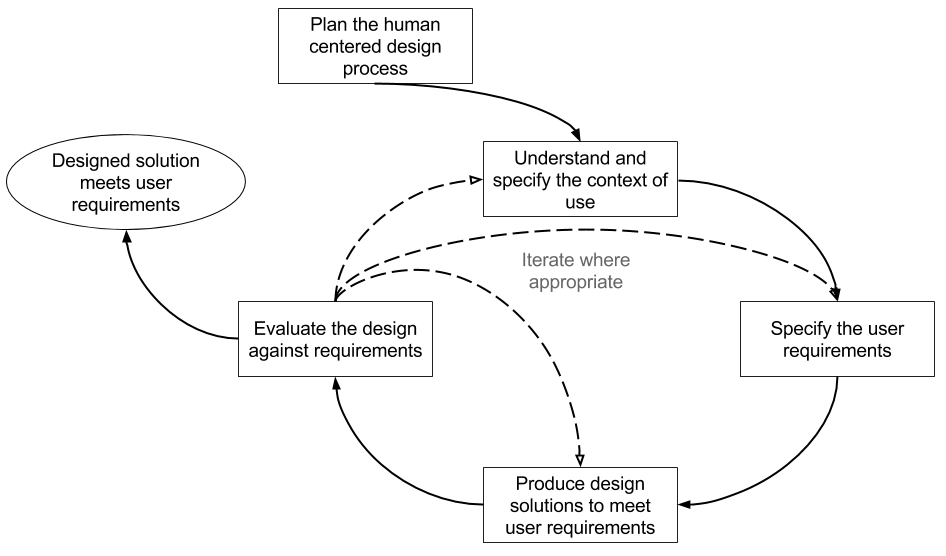
\includegraphics[width=1.0\textwidth]{figs/iterative-design-process.png}
  \caption[User-centered design process]{User-centered design process (adapted from: \cite{iso1999HCD}).}
  \label{fig:user-centered-design}
\end{figure}

System development during the Spring has followed a similar process as the user-centered design approach described above. Requirements were specified by the \gls{cmb} team, and a design prototype were developed and tested on possible end-users. Users were asked if they liked the new feature and they were also presented with the old user interface for comparison. If the test users liked the new feature it was accepted, otherwise it was further developed or revised until accepted. \\

Test users included supervisors, project team members, and randomly selected test users. Both the admin interface and user interface features were tested according to the above process. Future developers are advised to follow a user-centered design approach such as the Lean Startup methodology \cite{ries2011}, which has become fairly popular during the last few years.

%\subsection{Admin Interface Assessment}
%Some system administrators were also asked to assess the usability of the improved admin interface. The admin interface usability assessment was not a part of the user test, as the user test focused on testing the frontend interface used by normal users. We also have an restrictive amount of system administrators which has been trained in how to use the interface, which makes a test of the admin interface on a wast amount of participants unnecessary.


%\subsection{Validity}
%\paragraph*{Admin Interface Assessment} \hfill \\
%The number of admin users are small and might not be statistically significant. However, since the number of admin users is small and will stay small for some time in the future, it is important that the few admin users we have like the new admin interface improvements. Consequently, the assessment will likely be affected with experience from and observations done in the old admin interface. To improve the credability of the results one could also include testing of the admin interface in the optimal user test described above. However, this would make the user test more extensive and harder to execute, and would require a lot of administrative work.

\section{User Experiment}
\label{sec:user-testing}

\subsection{Motivation}
A user test was performed in the Specialization project and the project report were delivered in December 2015 as mentioned in Sub-\Cref{subsec:related-proj}. The \gls{cmb} system was one of three tools used by the students in mandatory assignments, where the \gls{cmb} system mainly was used for testing the system on more users then previously attempted by Follan and Støa \cite{mt:T&S}. The course assignments cover various topics and methods of producing parallel code in C++, like OpenMP, NEON, MPI and CUDA, and is about 25\% of the workload during the semester for the avarage student. The TDT4200 course staff added in total 5 programming problems to \gls{cmb} which were solvable by students, and the system received a lot of submissions during the semester. \\

During November of 2015 a total of 37 students delivered an optional questionnaire which included some questions about the \gls{cmb} system. In addition to the questionnaire, some feedback on the system was gathered during the last lecture of the course late in November. The feedback were mainly focused on usability aspects of the system, which helped the \gls{cmb} project team to discover bugs, and to setup and prioritize features to implement next. The prioritized list generated a backlog, which was used as a motivation when constructing the objectives presented in \Cref{sec:ps-inter}. \\

As this thesis potentially has improved system usability, it is interesting to conduct a user study to compare the usability of the two system versions. As mentioned in \Cref{sec:cmb}, the system developed by Follan and Støa will be refered to as system version one, while the updated system presented in \Cref{ch:imrpovements} will be refered to as system version two in the below discussion. As mentioned in \Cref{ch:design}, usability is a broad term and this thesis has contributed mainly against improving efficiency, learnability, and satisfaction of users as discussed in the mentioned chapter and implemented in \Cref{ch:improvements}. The above observation makes it interesting to test the following hypothesis:

\paragraph*{Hypothesis 1:} The usability, in terms of either efficiency, learnability, or user satisfaction, is higher in version two compared to system version one. \hfill \\

Further, it is interesting to investigate if the overall usability of the system has increased in the \gls{cmb} system version two i.e:

\paragraph*{Hypothesis 2:} The overall usability of system version two is higher compared to system version one. \hfill \\

\subsection{Methodology}
\label{sub-sec:user-testing-methodology}
The user test were conducted April 18th this Spring assesses the system improvements presented in \Cref{ch:improvements} with focus on usability. The goal of this second test is to further improve the results received from Specialization project user test or user test one. The second test required an interest in programming and programming experience from the participants, but no prior knowledge of C or C++ or any parallel programming libraries were set as a requirement to participate in the test. \\

The weak requirements were set since there were generally little interest from students in participating in the test. The low interest in the test is most likely due to bad timing, as many students have several assignment deliverables before the last lectures in mid April. Further, attracting students or others to participate in a user test for a master thesis is generally hard if the test takes several hours. \textit{As the focus of this test were to test the usability of the system, it should be sufficient for participants to have general knowledge and interest in programming to access system usability}. \\

The user test described a set of tasks to be completed by each participant. Since we are comparing the two system versions, the test does not assess the new features implemented and is assumed covered by \Cref{sec:cont-user-testing}. Appendix \ref{apdx:usertest} presents the tasks executed by every participant during the test, along with a questionnaire each participant were to complete before finishing the user test. \\

Nearly all participants conducted the test simultaneously in a lecture hall to simulate the heavy submission traffic we experienced before assignment deadlines in TDT4200. A couple of participants started the user test late or participated a couple of days after the official user test, to simulate the students in TDT4200 that experienced little or no traffic. Participants were informed that questions related to how to complete a task would not be answered during the test and that tasks should be completed individually. They were also informed that they could abort the test at any time. \\

\begin{table}
    \centering
    \begin{tabular}{ | l | p{6cm} |}
    \hline
    \textbf{Problem Name} & \textbf{Problem Description Summary} \\ \hline
    Hello World & Print out "Hello World!"". \\ \hline
    Digits & \textit{T} test cases are given as input, each test case describing the range between two numbers \textit{N} and \textit{M}. For each test case, output the number of zeroes present in all the numbers in the range [\textit{N}, \textit{M}]. \\ \hline
    Prime Number & For every number in the input, output if the number is a prime. \\ \hline
    WERTYU & For every encrypted input string, decrypt it and output the decrypted string. Hint: The input strings are encrypted with an QWERTY keyboard shifted one character to the right. \\ \hline
    Reverse String & For every input string output the reversed string. \\
    \hline
    \end{tabular}
    \caption{Available solvable problems during user test.}
    \label{tab:avail-prob}
\end{table}

The most time consuming task the participants had to complete were to submit code to one of the problems presented in Table \ref{tab:avail-prob}. Submitting code to problems is the core of the \gls{oj} and the process of uploading and running submissions were the most common procedure done by TDT4200 students. The procedure and aspects related to submissions was also mentioned the most times in feedback given by the TDT4200 students, and was therefore chosen as one of the main tasks to perform in this user test. Before starting the user test, the participants were also notified to comment extensively on the procure when filling out the survey. \\

The participants who were unfamiliar with C and C++ were given 5 different source files to the ``Prime Number''-problem which they were to submit to the system. The thought behind handing out source files, were to simulate that the participants made a number of tries before arriving at the correct solution. The ``Prime Number''-problem were chosen as it is of medium to easy difficulty. Participants who knew either C or C++ were also motivated to try to solve more than one problem if they arrived at a solution quickly, to extensively test the procedure of uploading and running submissions. Other tasks executed by participants included sign-up, login, viewing submissions and highscore lists, joining groups, creating and administering groups, and changing user e-mail and password. \\

The questionnaire found in Appendix \ref{apdx:usertest} contains the same questions about the \gls{cmb} system presented in the questionnaire given to the students in TDT4200. The questionnaire is, as mentioned in the Specialization project report, inspired a by typical Likert scale form developed by IBM\footnote{See: \url{http://garyperlman.com/quest/quest.cgi}} and complemented with textual based questions. To compare the results of the two questionnaires, it is important that they cover the same aspects and all questions developed in the Specialization project is therefore reused in the questionnaire handed out in this user study. In addition, a couple of extra multiple choice questions were added to the questionnaire of this test for the sake of clarity. \\

Likert scale questions are often used in usability assessment of software systems. In this test, the number of Likert scale alternatives is set to five per question. Each row in Table \ref{tab:likert-scale} shows the possible alternatives for a given question type, as well as each alternatives' corresponding score ranged from one to five. The answers to Likert scale values of the two user tests are then compared using statistical analysis as explained in Sub-\Cref{sub-sec:user-test-statistics}. To make it easier for participants to describe their thoughts about system features, the textual based questions are provided in the questionnaire and is further used as qualitative support when discussing the user study results.

\begin{table}[t!]
    \centering
    \begin{tabular}{ | c | p{1.5cm} | p{1.5cm} | p{1.5cm} | p{1.5cm} | p{1.5cm} |}
    \hline
    \multirow{2}{*}{\textbf{Question Type}} & \multicolumn{5}{ c| }{\textbf{Likert Score Range}} \\ \cline{2-6}
      & 1 & 2 & 3 & 4 & 5 \\ \cline{1-6}
    A & Very poor & Poor & Neutral & Good & Very good \\ \hline
    B & Strongly disagree & Disagree & Neither agree or disagree & Agree & Strongly agree \\ \hline
    C & Very hard & Hard & Neutral & Easy & Very easy \\ \hline
    D & Not satisfied at all & A~little bit~satisfied & Neutral & Satisfied & Very satisfied \\ \hline
    \end{tabular}
    \caption{Likert scale alternatives on question type.}
    \label{tab:likert-scale}
\end{table}

\subsection{Statistical Analysis}
\label{sub-sec:user-test-statistics}
The tool Gnumeric \cite{GNUMERIC} is used for statistical data analysis comparison on the multiple choice results of the two user tests. The results are reproducible using the pie charts and number of participants of each user test found in Appendix \ref{apdx:usertest}. Each multiple choice answer from both tests are translated into the corresponding Likert scale value, and values of matching questions between the two user tests are then compared. To simplify the discussion of results and validity, the user test conducted as part of the Specialization project will be referred to as user test one or T1 and the user test conducted in this thesis will be referred to as user test two or T2. \\

A F-test \cite{moore2007} is conducted to determine if the compared data set variances can be considered equal. The F-test calculates a P-value, which is a measurement of how extreme the results of a given test are relative to the underlying statistical model. The P-value is compared to a defined significance level, and variances are considered equal if the P-value is less then the decided significance level or unequal if the P-value is bigger than significance level. The result can also be formulated as keeping the null hypothesis ($H_0$), while the opposite situation are referred to as rejecting the null hypothesis and accepting the alternative hypothesis ($H_1$). \\

A T-test \cite{walpole1993} is performed on each question to determine if two user tests have significantly different means. The T-test can be executed either assuming equal or unequal variances, and the result of the F-test determines which version of the T-test to execute. The T-test also outputs a P-value which is used in the same way as explained in the above paragraph. \\

The statistical analysis in this thesis assumes a significance level ($\alpha$) of 5\%. Further, the null hypothesis ($H_0$) for the T-test assumes equal means of the two datasets, while the alternative hypothesis ($H_1$) is set depending on if we are conducting either a one-tailed or two-tailed T-test. Equation \ref{eq:h1-t-test} shows the possible alternative hypothesis for the T-test, where $\mu_{1}$ and $\mu_{2}$ are the means for user test one and two respectively. In this thesis we use the one-tailed alternative hypothesis, as we want to obtain stronger results for system version two.

\begin{equation} \label{eq:h1-t-test}
   H_1 =
    \begin{cases}
        \mu_{2} > \mu_{1} & \quad \text{if one-tailed test}\\
        \mu_{1} \neq \mu_{2} & \quad \text{if two-tailed test}\\
    \end{cases}
\end{equation}

If the T-test indicates a significant difference between the two user groups further analysis is needed. If so, an Anderson-Darling test \cite{razali2011} is performed to check the normality of the data sets, as normality is often a requirement for a valid T-test. However, if the normality check fails, the non-parametric \gls{wmw} test \cite{hodges2005} is performed on each of the question groups accepted by the T-test. The test is used to support the conclusion of the T-test, as non-parametric tests are often used when the compared data sets are non-normally distributed. \\

The statistical effect-size is also reported and used when discussing the results. The effect-size is meant by the statistical \textit{strength} of a result, and will be important in our discussion of the multiple choice results. The reported effect-size metrics used is Cohen's d, Hedge's g, and Pearson's r \cite{cumming2013}.\footnote{Calculated with this tool: \url{http://www.polyu.edu.hk/mm/effectsizefaqs/calculator/calculator.html}.} Cohen's d is often used as effect size to measure the strength of a t-test, as well as Person's r which is a well known effect-size metric. Hedge's g is also included in the results, as it is more accurate than Cohen's d with small sample sizes. Table \ref{tab:effect-size} reports the strength scale for each of the used effect-size metrics, and a conclusion from a test is considered stronger the higher effect-size reported. \\

Cohen's d and Hedge's g is also used to calculate the statistical \textit{power} of a conclusion. Statistical power is the probability of correctly rejecting $H_0$ when $H_1$ is true, and is important when discussing threats against validity to be sure that we have enough respondents to draw valid conclusions. Statistical power of the t-test is calculated using the Real Statistics Resource Pack in Microsoft Excel \cite{RSRP}.

\begin{table}[t!]
    \centering
    \begin{tabular}{ | c | c | c | c |}
    \hline
    \textbf{Effect size} & \textbf{Pearson's r} & \textbf{Cohen's d} & \textbf{Hedge's g} \\ \hline
    Small & 0.1 & 0.2 & 0.2 \\ \hline
    Medium & 0.3 & 0.5 & 0.5 \\ \hline
    Large & 0.5 & 0.8 & 0.8 \\ \hline
    \end{tabular}
    \caption{Effect sizes and corresponding metric values.}
    \label{tab:effect-size}
\end{table}

\subsection{Results and Evaluation}
\label{sub-sec:user-testing-results}
There were in total 21 participants in the second user test. Table \ref{tab:label-to-title} shows a mapping between questions question titles and question labels, which makes it easier to reference the questions in the below discussion. As mentioned, there were a total of 37 TDT4200 students providing feedback in the optional questionnaire given during the Autumn semester. The pie-charts and a summary of textual based feedback for both the user test one and two can be found in Appendix \ref{apdx:usertest}. All statistical test results reported in tables are rounded to three decimal places if applicable, that is, results are not rounded if it changes the outcome of the below discussions. \\

Table \ref{tab:results-tests-all} shows the means and variances of user test one and two responses for each Likert scale question in common for the two user tests. The table also include F-test P-values and the conclusion of the F-test compared to the significance level, which determines to either assume equal or unequal variances when performing the T-test. The T-test P-value is also reported, and is used to determine if a rejection of null hypothesis is needed. \\

The three questions \texttt{A3}, \texttt{D1}, and \texttt{A4} should reject $H_0$ as indicated by the T-test results in Table \ref{tab:results-tests-all}. However, none of the data sets are normally distributed according to the Anderson-Darling test. Subsequently, a \gls{wmw}-test is conducted to support the conclusion of the T-test. Table \ref{tab:significant-results} reports the resulting P-value of the \gls{wmw}-test, as well as effect-sizes and power calculations. \\

\begin{table}[t!]
    \centering
    \begin{tabular}{ | c | p{9cm} |}
    \hline
    \textbf{Label} & \textbf{Question Title} \\ \hline
    \texttt{O1} & ``What year of study are you in?'' \\ \hline
    \texttt{O2} & ``Which of the following best describes your study programme?''  \\ \hline
    \texttt{A1} & ``How would you rate the Climbing Mont Blanc system in general?'' \\ \hline
    \texttt{B1} & ``It was easy to use the system?'' \\ \hline
    \texttt{A2} & ``How would you rate the usability of the Climbing Mont Blanc system?'' \\ \hline
    \texttt{C1} & ``Was it difficult to learn how to use the Climbing Mont Blanc system?'' \\ \hline
    \texttt{A3} & ``How would you rate the design of the Climbing Mont Blanc user interface?'' \\ \hline
    \texttt{C2} & ``How would you rate the process uploading and running a program?'' \\ \hline
    \texttt{D1} & ``How satisfied are you with the feedback given by the Climbing Mont Blanc system?'' \\ \hline
    \texttt{B2} & ``The feedback given by the system is clear and helpful?'' \\ \hline
    \texttt{A4} & ``How would you rate the information on the HowTo-page?'' \\ \hline
    \end{tabular}
    \caption[Label to question title mapping]{Label to question title mapping: Labels are created according to Table \ref{tab:likert-scale}. Questions marked \texttt{O*} are meant as other questions not within the five point Likert scale range.}
    \label{tab:label-to-title}
\end{table}

The \gls{wmw}-test also indicate significant results as its P-values are lower than $\alpha$. Question \texttt{D1} has the most significant results, as the effect-size is large and the power is high using both Cohen's d and Hedge's g. Using Hedge's g to compute power, we can by a 97.2\% probability be certain that we have correctly rejected $H_0$ when $H_1$ is true. We can therefore conclude that users, most probably, are more satisfied with the feedback of the system version two. The results reported for question \texttt{B2} in Appendix \ref{apdx:usertest} also indicates that feedback is good, as over 80\% of participants either agree or strongly agree that the feedback given by the system is clear and helpful.  \\

\begin{table}[t!]
    \centering
    \begin{tabular}{|c||c|c||c|c||c|c||c|c||}
      \hline
      \multirow{2}{*}{\textbf{Question}} & \multicolumn{2}{ |c|| }{\textbf{A1}} & \multicolumn{2}{ |c|| }{\textbf{A2}} & \multicolumn{2}{ |c|| }{\textbf{C1}} & \multicolumn{2}{ |c|| }{\textbf{A3}} \\ \cline{2-9}
      &  T1 & T2 & T1 & T2 & T1 & T2 & T1 & T2 \\ \hline
      \textbf{Mean} & 3.676 & 3.857 & 3.730 & 3.809 & 3.919 & 3.905 & 3.730 & 4.143 \\ \hline
      \textbf{Variance} & 0.392 & 0.429 & 0.592 & 0.162 & 0.521 & 0.590 & 0.369 & 0.329 \\ \hline
      \textbf{F P-value} & \multicolumn{2}{c||}{0.396} & \multicolumn{2}{c||}{0.002} & \multicolumn{2}{c||}{0.362} & \multicolumn{2}{c||}{0.400} \\ \hline
      \textbf{Variance} & \multicolumn{2}{c||}{Equal} & \multicolumn{2}{c||}{Unequal} & \multicolumn{2}{c||}{Equal} & \multicolumn{2}{c||}{Equal} \\ \hline
      \textbf{T P-value} & \multicolumn{2}{c||}{0.151} & \multicolumn{2}{c||}{0.303} & \multicolumn{2}{c||}{0.472} & \multicolumn{2}{c||}{0.002}\\ \hline
      \textbf{Reject $H_0$?} & \multicolumn{2}{c||}{No} & \multicolumn{2}{c||}{No} & \multicolumn{2}{c||}{No} & \multicolumn{2}{c||}{Yes}\\ \hline
    \end{tabular} \\[5pt]
    \begin{tabular}{|c||c|c||c|c||c|c||}
      \hline
      \multirow{2}{*}{\textbf{Question}} & \multicolumn{2}{ |c|| }{\textbf{C2}} & \multicolumn{2}{ |c|| }{\textbf{D1}} & \multicolumn{2}{ |c|| }{\textbf{A4}} \\ \cline{2-7}
      &  T1 & T2 & T1 & T2 & T1 & T2 \\ \hline
      \textbf{Mean} & 3.595 & 3.524 & 2.568 & 3.619 & 3.324 & 3.842 \\ \hline
      \textbf{Variance} & 0.970 & 0.762 & 0.919 & 0.947 & 0.892 & 0.474 \\ \hline
      \textbf{F P-value} & \multicolumn{2}{c||}{0.287} & \multicolumn{2}{c||}{0.454} & \multicolumn{2}{c||}{0.060}\\ \hline
      \textbf{Variance} & \multicolumn{2}{c||}{Equal} & \multicolumn{2}{c||}{Equal} & \multicolumn{2}{c||}{Equal} \\ \hline
      \textbf{T P-Value} & \multicolumn{2}{c||}{0.393} & \multicolumn{2}{c||}{$9.6x10^{-5}$} & \multicolumn{2}{c||}{0.022} \\ \hline
      \textbf{Reject $H_0$?} & \multicolumn{2}{c||}{No} & \multicolumn{2}{c||}{Yes} & \multicolumn{2}{c||}{Yes} \\ \hline
    \end{tabular}
    \caption{Mean, variance, F-test, and T-test results.}
    \label{tab:results-tests-all}
\end{table}

The questions \texttt{A3} and \texttt{A4} is also accepted by both the T-test and \gls{wmw}-test. However, their strength in terms of all effect-size metrics indicates medium strength for \texttt{A3} and low to medium strength for \texttt{A4}. The statistical power of question \texttt{A3} and question \texttt{A4} should have been higher for us to draw any valid conclusions. We can only conclude that system version two might have a better user interface design and an improved HowTo-page. \\

The overall usability is good in both system versions. This also corresponds to the conclusion of tests ran against question  \texttt{C1}, and answers to textual based feedback received from both user test one and user test two. There is also generally little overlap in textual based feedback, which indicates that there have been some improvements to usability. Some of the textual based feedback, such as adding language versions and project information to the HowTo-page as proposed in \Cref{sec:impr-proposals}, has already been noted by the \gls{cmb} team and is already listed in the backlog found in Appendix \ref{apdx:backlog}. \\

The textual based questions are as mentioned meant as support for the multiple choice questions. The questions are also important for the future development of the \gls{cmb} prototype. Proposals of new features, such as low-level noice in timing measurements, multi file uploads, and updated feedback on run queue index have been noted by the \gls{cmb} team. New feature proposals is marked in the backlog in Appendix \ref{apdx:backlog}, and \Cref{sec:future-work} present proposals of possible next steps in the project. \\

Some of the feedback noticed by participants, such as real-time updates of submission placement in the run-queue, was actually in the making shortly before the conduction of the user experiment. As the improvements showed to be more extensive to implement than first thought, they were not implemented. The choice was made as it was little time to develop unit tests and test the implementation before the conduction of the user test, and the features also required changes to backend code which was the domain of another master student. \Cref{ch:evaluation} further discusses the matter. \\

The experiment results indicates that users are more satisfied with version two of the system. Users are from the above study more satisfied with the feedback given by system version two, and there is also a trend towards users being more satisfied with the user interface design and the information displayed at the HowTo-page. We can therefore conclude that it is likely that usability in terms of either efficiency, learnability, or user satisfaction is better in version two of the system i.e Hypothesis 1 seem to be true. \\

Likert scale questions covering overall usability does not indicate a significant improvement in this experiment. Both test one and test two indicated good overall usability i.e we can not conclude that Hypothesis 2 is true. However, users were only testing actions in common of the two system versions. New features implemented during the Spring were not included in this experiment, but is considered covered by the continuous user testing described in \Cref{sec:cont-user-testing}. Since the range of possible actions against the system has increased in version two and users has approved the new features, we can to some extent also argue that the overall usability has improved.

\begin{table}[t!]
    \centering
    \begin{tabular}{|c||c||c||c||}
      \hline
      \textbf{Question} & \textbf{A3} & \textbf{D1} & \textbf{A4} \\\hline
      \textbf{WMW P-value} & 4.231\% & 0.081\% & 4.400\%  \\ \hline
      \textbf{r} & 0.330 & 0.478 & 0.283\\ \hline
      \textbf{d} & 0.699 & 1.088 & 0.590 \\ \hline
      \textbf{g} & 0.684 & 1.076 & 0.557\\ \hline
      \textbf{Power (using d)} & 0.711 & 0.975 & 0.564 \\ \hline
      \textbf{Power (using g)} & 0.692 & 0.972 & 0.518 \\ \hline
    \end{tabular}
    \caption{Wilcoxon-Mann-Whitney P-values, effect-sizes, and power results.}
    \label{tab:significant-results}
\end{table}

%\begin{table}[t!]
%    \centering
%    \begin{tabular}{cc|c|c|c|c|c|c|c|c|}
%      \hline
%      \multicolumn{2}{ |c| }{\textbf{Question}} & \textbf{Mean} & \textbf{Variance} & \textbf{F} & \textbf{F Crit} & \textbf{One-tailed?} & \textbf{T stat} & \textbf{T crit} & \textbf{Reject $H_0$?} \\ \hline
%      \multicolumn{1}{ |c  }{\multirow{2}{*}{\textbf{A1}} } &
%      \multicolumn{1}{ |c| }{T1} & 3,676 & 0,392 & \multirow{2}{*}{1,904} & \multirow{2}{*}{1,870} & \multirow{2}{*}{No} & \multirow{2}{*}{1,031} & \multirow{2}{*}{2,021} & \multirow{2}{*}{No}  \\ \cline{2-4}
%      \multicolumn{1}{ |c| }{}                    &
%      \multicolumn{1}{ |c| }{T2} & 3,857 & 0,429 & & & & & &    \\ \hline
%    \end{tabular}
%    \caption{Mean, Variance, F-test, and T-test results multiple choice questions}
%    \label{tab:result-tests-all}
%\end{table}


\subsection{Threats to Validity}
\label{sub-sec:user-test-validity}
Conclusion validity concerns to what extent conclusions from statistical analysis are correct. It is closely related to statistical power, and is important when concidering to reject $H_0$. In statistical analysis we typically have false negatives or false positives. False positives (called Type I errors) means a significant results are found even though data indicates otherwise, for example due to too few participants. Further, false negatives (called type II error) can be present which means that $H_0$ is not rejected even though there could have been an effect with a larger number of participants. In the below discussion we will assume we at least want a power of 80\%, to be sure that a conclusion is correct. \\

Question \texttt{D1} seems to be a valid conclusion. We could actually had a power of 80\% with only 20 participants in user test one and 12 participants in user test two to draw a valid conclusion from the results.\footnote{Calculated using this tool: \url{http://www.biomath.info/power/ttest.htm}.} Question \textit{A3} has too few participants to draw a valid conclusion, however there is a trend indicating a better scored satisfaction over the new user interface. We would have reached our target statistical power with 47 participants in user test one and 27 participants in user test two. However, satisfiability in system design is only one aspect of usability and we also need to keep in mind that participants were only testing a sub set of the new features in the system. \\

Question \textit{A4} had statistically lowest power of the three questions having statistically significant results. The power at 51.7\% using Hedge's g is not strong enough to draw a valid conclusion. We would have needed 70 participants in test one and 40 participants in test two to correctly accept $H_0$. However, improvements to the HowTo-page is listed as secondary improvements in the objectives listed in \Cref{sec:ps-inter}, and the small changes made presented in \Cref{sec:impr-proposals} were due to the usage of the system in a learning experiment. \\

Construct validity concerns if the experiment actually measure what it declares to measure \cite{Cronbach1955}. The user experiment tried to measure if there were any improvements to usability in system version two. As mentioned, some questions were added to the questionnaire this Spring which could potentially damage the validity of results. However, these were only added for clarity and should not damage the conclusions made above. Also, participants might have had trouble assessing usability as they might have used a long time developing code instead. However, participants were given the option of receiving a set of programs simulating multiple tries against the system before arriving at the correct solution. \\

Internal validity concerns if there is a causal correspondence between the methodology used and the results of the experiment \cite{Oates2006}. If there are other factors, or confouncding variables, in the experiment which leads us to the same conclusions, the measurements has poor internal validity. There are some factors in the above experimental setup that may threaten the internal validity of the results. \\

Participants in the second user test does not necessarily have the same background and interests as the participants of the first user test. This may have an effect on how the participants percieve the system, and it may be different from the perception made by students students in TDT4200. Also, some participants of the second user test were not familiar with C or C++, and received a set of executables for a programming problem to simulate normal system users. The goal of this user test were to test system usability and not programming skills or personal interests, and both groups of participants also had the same foundation when starting to use the system.  \\

Participants in user test two also used the system for a short period of time compared to participants in user test one. The participants in user test two may not have been able to test the system thoroughly like the students in TDT4200 had a chance to do, as they used the system in a total of 5 exercises throughout the Autumn semester. Participants in user test one might therefore have more experience in using the system. However, participants in the second user test were adviced to test the system thouroghly if they finished early.\\

Many of the participants are friends of or familiar to the \gls{cmb} team. They were invited due to low interest in the user experiment. Participants familiar to the system or \gls{cmb} team might effect the above results further in either a positive or negative way. The participants were therefore kindly asked to give as objective feedback as possible. In order to strengthen the above statistical analysis more research can be conducted. \\

External validity concerns the generalizability of measurements and results \cite{Oates2006}. The participants who conducted the second user test were familiar to the \gls{cmb} team, and some also had little interest in parallel programming or C/C++ programming. More research needs to be conducted in order to determine if the improvements are generalizable to cover programmers interested in low-level parallel programming. It is also worth mentioning the difference in distribution of year of study, were most participants in user test two are 5th year students apposed to 4th year students in user test one. A further discussion of possible test setups is presented in \Cref{sec:eval-user-testing}. Regardless of participants' background, the results of the experiment is interesting and we have hopefully made more programmers aware of heterogeneous programming and \gls{oj} systems. \\

\section{System Unit Tests}
\label{sec:system-unit-tests}
This section will present the statement coverage of system unit tests. A high test coverage is important to ensure correct functionality, and allows quick detection of features that breaks system functionality during development. Unit tests were developed during implementation of the system improvements described in \Cref{ch:improvements}, and are reported to demonstrate the correctness of developed code and the resulting system. This thesis has a goal of 90\% test coverage for the system as introduced to the project by Follan and Støa \cite{mt:T&S}. \\

The reader should be aware that the unit tests developed by Follan and Støa is also included in the below presentation of coverage. This thesis has only developed or extended unit tests for the system improvements presented in chapter \ref{ch:improvements}. This section cencerns the correctness of improved functionality in a working system, and reader should refer to the Master Thesis of Follan and Støa for an overview of previously developed functionality and in detail test coverage of that functionality.  \\

Information about how to run system unit tests and generate coverage reports can be found in Appendix \ref{apdx:setup}.

\subsection{Frontend}
\begin{table}[h!]
    \centering
    \begin{tabular}{c c c c}
      \hline
      \textbf{Directory} & \textbf{Statements} & \textbf{Statements covered} & \textbf{Coverage} \\ \hline
      \textit{config/} & 1 & 1 & 100\% \\
      \textit{controllers/} & 759 & 676 & 89\% \\
      \textit{directives/} & 78 & 9 & 12\% \\
      \textit{services/} & 33 & 19 & 58\% \\ \hline
      \textbf{Total} & 871 & 705 & 81\% \\ \hline
    \end{tabular}
    \caption{Frontend total test coverage.}
    \label{tab:frontend-coverage-all}
\end{table}

The frontend unit tests are developed in Jasmine \cite{JASMINE} as mentioned in \Cref{sec:cmb-ci}. Also, Karma \cite{KARMA} is used as test runner to develop the coverage reports, and Gulp \cite{GULP} is used to launch the Karma test runner.  \\

Table \ref{tab:frontend-coverage-all} shows the coverage of all files for the frontend code. The overall test coverage is under 90\% as set above. However, as mentioned by Follan and Støa, the low coverage is due to missing tests to third-party code in the \textit{directives/} directory, and is only used to give colored feedback of password strength during sign up which is not vital for the overall functionality of the system. \\

The \textit{services/} directory also has low code coverage and is below the 90\% requirement. The low coverage is mainly due to the implemented bulletin functionality presented in \Cref{sec:impr-frontend}. The unit test covering the bulletin functionality is not complete, as it would require us to expose private functions within the bulletin component in order to write a unit test with good coverage. Instead of exposing private functions just for the sake of the unit tests, the component were tested manually. It is also worth mentioning that the component is not crucial for overall system functionality. \\

The components containing most of the frontend functionality is found in the \textit{controllers/} directory. The coverage of 89\% overall is a result of the 82\% coverage of the \textit{problem.js} controller. The missing statements to be covered by test is mainly event based code, such as file upload and Socket.io events, and requires unit tests to trigger fake events. While triggering fake events can be done in unit tests, the callback function\footnote{A function passed as an argument to second function, which is called during execution of the second function.} of the event runs code covered by other unit tests and developing unit tests to cover event based code were therefore considered less important. By disregarding the coverage of event based code, the coverage of the frontend should be above the 90\% requirement.

\begin{table}[t!]
    \centering
    \begin{tabular}{c c c c}
      \hline
      \textbf{Controller} & \textbf{Statements} & \textbf{Statements covered} & \textbf{Coverage} \\ \hline
      \textit{error\_msg.js} & 21 & 21 & 100\% \\
      \textit{forgot\_password.js} & 9 & 9 & 100\% \\
      \textit{group.js} & 63 & 58 & 92\% \\
      \textit{home.js} & 32 & 28 & 88\% \\
      \textit{leader.js} & 81 & 72 & 89\% \\
      \textit{leader\_problem\_stats.js} & 70 & 67 & 96\% \\
      \textit{leader\_user\_stats.js} & 45 & 42 & 93\% \\
      \textit{login.js} & 12 & 12 & 100\% \\
      \textit{logout} & 11 & 11 & 100\% \\
      \textit{navbar.js} & 3 & 3 & 100\% \\
      \textit{newgroup.js} & 17 & 17 & 100\% \\
      \textit{problem.js} & 323 & 265 & 82\% \\
      \textit{profile.js} & 54 & 53 & 98\% \\
      \textit{signup.js} & 18 & 18 & 100\% \\ \hline
      \textbf{Total} & 759 & 676 & 89\% \\ \hline
    \end{tabular}
    \caption{Frontend controller test coverage.}
    \label{tab:frontend-coverage-controllers}
\end{table}

\subsection{Server}
Table \ref{tab:server-module-coverage} shows the unit test coverage for the server code. The coverage of the server code is at 90\%, which is therefore an accepted level of coverage. However, the coverage can be further improved by extending by improving the coverage of modules \textit{cmb\_utils.helpers} and \textit{cmb\_utils.wrappers}. \\

The unit tests does not cover some of the methods performing \gls{os} calls in module \textit{cmb\_utils.helpers}. \gls{os} calls are often simulated (mocked) in unit tests, as \gls{os} calls often take some time to execute and we want unit tests to execute as fast as possible. As the unit tests mock away most functionality of \gls{os} calls, these unit tests had a low priority and were instead tested manually. \\

The module \textit{cmb\_utils.wrappers} contains checks to validate session tokens and has the lowest unit test coverage. The missing unit test needs to test exception states which can occur, and has not been implemented. These unit tests has not been a prioritized, as the functionality has been extensively tested by Follan and Støa, and is also tested automatically during normal use of the system. \\

It is also worth mentioning that Flask-SocketIO event module is not covered by the unit tests. As testing of the module involves multiple components of the system, that is, both the server, frontend, and their interaction, the tests can instead be concidered as integration tests. Integration testing has been performed manually both locally and at the \gls{cmb} development server, and the module is thus not included in Table \ref{tab:server-module-coverage}. However, future developers should consider adding automatic integration tests at some later point, to lower the amount of manual testing needed before deploying to production.

\begin{table}[h!]
    \centering
    \begin{tabular}{c c c c}
      \hline
      \textbf{Module} & \textbf{Statements} & \textbf{Statements missing} & \textbf{Coverage} \\ \hline
      \textit{admin.admin} & 150 & 28 & 81\% \\
      \textit{cmb\_utils.helpers} & 86 & 17 & 80\% \\
      \textit{cmb\_utils.mail} & 5 & 0 & 100\% \\
      \textit{cmb\_utils.wrappers} & 50 & 15 & 70\% \\
      \textit{database.models} & 168 & 10 & 94\% \\
      \textit{routes.bulletin} & 21 & 0 & 100\% \\
      \textit{routes.groups} & 208 & 3 & 99\% \\
      \textit{routes.problems} & 21 & 12 & 95\% \\
      \textit{routes.submissions} & 150 & 14 & 91\% \\
      \textit{routes.users} & 93 & 3 & 97\% \\
      \textit{server} & 72 & 7 & 90\% \\ \hline
      \textbf{Total} & 1024 & 98 & 90\% \\ \hline
    \end{tabular}
    \caption{Server modules test coverage.}
    \label{tab:server-module-coverage}
\end{table}
